%%%%%%%%%%%%%%%%%%%%%%%%%%%%%%%%%%%%%%%%%%%%%%%%%%%%%%%%%%%%%%%%%%%%%%%%%%%%%%%%
%science.tex: Chapter on DM physics:
%%%%%%%%%%%%%%%%%%%%%%%%%%%%%%%%%%%%%%%%%%%%%%%%%%%%%%%%%%%%%%%%%%%%%%%%%%%%%%%%
\chapter{Dark Matter}
\label{chapter:dm}
%%%%%%%%%%%%%%%%%%%%%%%%%%%%%%%%%%%%%%%%%%%%%%%%%%%%%%%%%%%%%%%%%%%%%%%%%%%%%%%%

Many physicists throughout history have been puzzled by new phenomena, but the
confusion surrounding dark matter -- estimated to be roughly 85\% of the total
matter in the universe -- is surely one of the biggest puzzles. While many
astronomical observations at various scales have confirmed the existence of
dark matter, we have yet seen any observations of its particle interacting
with our detectors. This has ruled out many models for dark matter's particle
nature, but there are still many more available which can both explain the
current observations of dark matter gravitational and cosmological effects
while skirt the limitations defined by the \emph{lack} of observation in
particle experiments.

\section{Evidence for Dark Matter}

The first evidence physicists had for an unseen material floating throughout the universe
was the observation of galactic rotation curves \cite{rubin-rotationcurve-1980,rotationcurve-2000}.
These observations measure the speed of different stars within a galaxy and compare this speed to
the distance of that star from the center of the galaxy. We can calculate this relationship
using \gls{gr} \cite{rotationcurve-predictions-2007} and the
observations differ drastically from this calculation. The stars within galaxies we've observed move
much faster than \gls{gr} would predict (\cref{fig:rotation-curve}) leaving us with two explanations: either \gls{gr} is not the correct theory
to use in this situation or there is more un-seen mass floating within the galaxy allowing these stars
to move faster without leaving the galactic orbit.

Other indirect measurements give us additional ways to access information about this odd phenomena.
Within the framework of \gls{gr}, since energy and mass actually warp the fabric of spacetime,
we expect to see light itself follow a bent path around massive objects - a phenomenum that is called
\gls{grav-lens} and is observed and well modeled by \gls{gr}'s predictions \cite{gravlensing-2004}.
The accuracy of \gls{gr} within this context - a mass and distance scale similar to the rotation curve oddities also observed -
put more requirements on any modified theory of gravity that could both explain the rotation curves and gravitational lensing.
Additionally, measurements on some of the largest scales and from the early universe
display signs of a certain mass density attributed to non-baryonic matter.
\todo{bullet cluster figure}

The \gls{cmb} and \gls{bao} provide a method for deducing densities of various classes of matter
in the early universe. Gravity attracts while pressure from the squeezing of the plasma repules
which produces oscillations in the density of matter in space and time. These \gls{bao} are
imprinted on our snapshot of this early-universe plasma, the \gls{cmb}, which we can measure with
a high degree of accuracy and fit to various models of what existed at this time of the universe.
The best fit of these models corresponds to only $\sim 5\%$ of the mass density being normal matter
like we see today while the rest is composed of material that only significantly interacts gravitationally.
\todo{need citation and figure for cmb and bao}


\begin{itemize}
      \item Astronomy observations show lots of measurements
            \begin{itemize}
                  \item Type1a Supernovae \cite{type1a-supernova-2010}
                  \item Big Bang Nucleosynthesis \cite{nucleosynthesis-1998}
                  \item Probably not mini black holes \cite{constraints-primordial-black-holes-2021}
            \end{itemize}
      \item Can conclude pretty comfortably that DM exists
\end{itemize}

\begin{figure}
      \centering
      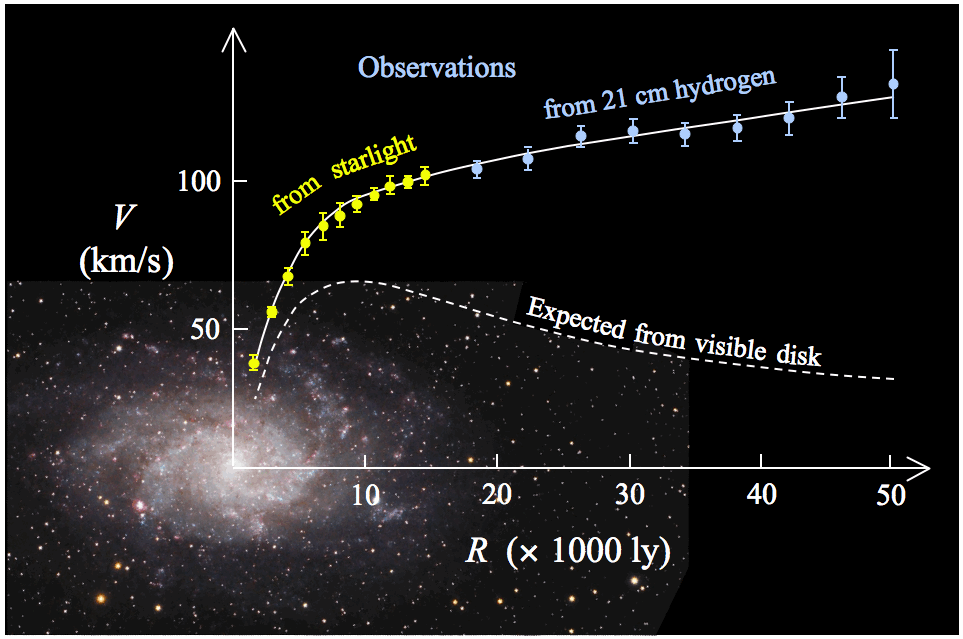
\includegraphics[width=0.6\textwidth]{figures/theory/rotation-curve-evidence-for-dm.png}
      \caption{
            Depiction of the velocity of stars within a galaxy as a function of their distance
            from the galactic center. The dotted line is a prediction of this relationship using
            \gls{gr} along with the mass tabulated from the visible starts while the data points
            (and the solid line fitted to them) are what are actually seen in galaxies today.
      }
      \label{fig:rotation-curve}
\end{figure}

\section{Particle Nature of Dark Matter}
The theoretical possibilities explaining dark matter are broad \cite{darksectors-2016}
event when excluding ourselves to the assumption that the dark matter phenomenum is explained
by the existence of a dark matter particle since the start of the start of the universe alongside
our normal matter particles. Here, I will refer to this particular dark matter
as \gls{dm} which, in general, needs to satisfy the following requirements.
\begin{itemize}
      \item \textbf{Dark} There has been no detection of these particles via the light observed with our telescopes;
            therefore, the dark matter has to not interact via the electromagnetic force.
      \item \textbf{Long Living} Measurements of \gls{dm}'s mass density and presence agree across time
            (from as early as the \gls{cmb} era), so \gls{dm} needs to have a long lifetime.
      \item \textbf{Observable Here} Measurements of \gls{dm} agree across different points in space,
            so it must be observable here on earth in some terresterial experiment.
      \item \textbf{Thermal Relic} Both \gls{dm} and standard matter have similar
            cosmological densities, so we expect some interaction (even a weak one) should connect their
            origins to the early universe allowing both to exist from the Big Bang.
      \item \textbf{Universal Density} Since we can indirectly measure a \gls{dm} mass density on
            cosmological scales, we impose the requirement that any \gls{dm} model needs to allow for
            this density.
\end{itemize}
Even with these assumptions and the requirements they imply, there still exist a plethora of
theoretical models that can satisfy all of them.

\begin{figure}
      \centering
      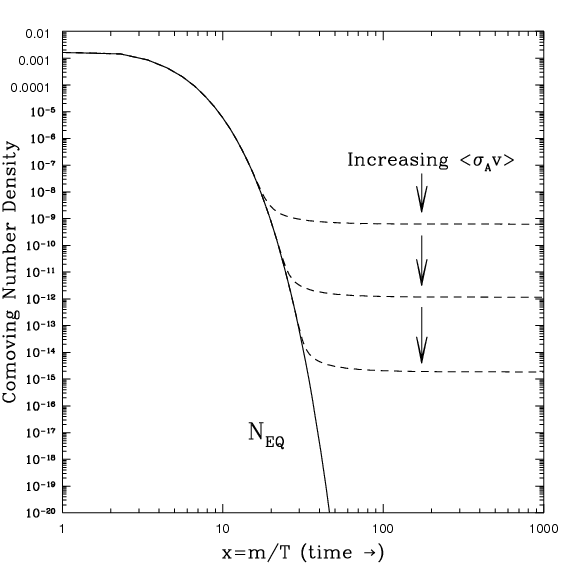
\includegraphics[width=0.5\textwidth]{figures/theory/number-density-at-freeze-out.png}
      \caption{
            From \cite{thermal-freezeout-diagram-1996}, the co-moving cosmological number density of \gls{dm} as a function of the universe
            temperature. As the universe cools, the number density decreases until the \gls{dm}
            becomes too sparse to interact with other \gls{dm} particles, ``freezing'' to a specific
            number density until today.
      }
      \label{fig:number-density}
\end{figure}

\begin{itemize}
      \item Whole lot of options
            \begin{itemize}
                  \item Thermal relic reminder (i.e. how mass gets connected to cross section due to universal density constraint) \cite{thermal-freezeout-diagram-1996}
                  \item Massive field loop causes dark and standard photon to mix
                  \item Details of model left to higher energies (EFT) $\rightarrow$ summarize it as a mixing parameter $\epsilon$ \cite{kinetic-mixing-1986}
                  \item But what happens to the dark photon after that? Could stay in "dark sector" (invisible decay) or return to standard particles (visible decay)
                  \item HPS focused on visible decays where the produced electron-positron pair's kinematics may rely on inner-workings of dark sector
                  \item Categorize dark sector models ("Vanila", SIMPs, iDM, others...)
            \end{itemize}
      \item Pseudo-Dirac iDM
      \item Motivations for complicated model
            \begin{itemize}
                  \item WIMPs pretty well constrained \cite{supercdms-2018,damic-2020,xenon1t-2018}
                  \item Direct detection is hard with LDM \cite{ldmconstraints-2019}
                  \item super-WIMPs at keV mass scale \cite{superwimps-2008}
                  \item iDM is interesting for others as well \cite{darkseaquest-2018}
            \end{itemize}
\end{itemize}

\begin{figure}
      \centering
      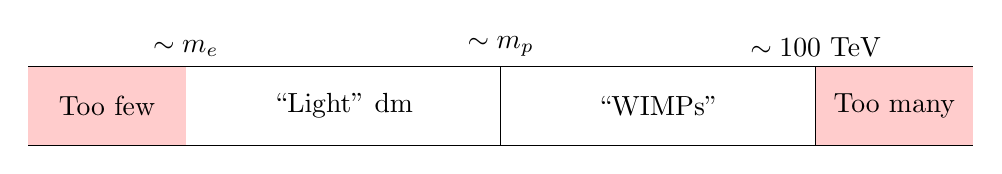
\begin{tikzpicture}
    % horizontal top/bottom lines
    \draw (0,0) -- (12,0);
    \draw (0,1) -- (12,1);
    % dividing lines along with relevant scale markers
    \draw (2,0) -- (2,1) node[above] {$\sim m_e$};
    \draw (6,0) -- (6,1) node[above] {$\sim m_p$};
    \draw (10,0) -- (10,1) node[above] {$\sim100~$TeV};
    % fill non-thermal ranges with light red
    \fill [red!20!white] (0,0) rectangle (2,1);
    \fill [red!20!white] (10,0) rectangle (12,1);
    % labels offering descriptions of ranges inside the boxes
    \node at (1,0.5) {Too few};
    \node at (4,0.5) {``Light'' \gls{dm}};
    \node at (8,0.5) {``WIMPs''};
    \node at (11,0.5) {Too many};
\end{tikzpicture}
      \caption{Mass scale of Thermal Relic \gls{dm}.}
      \label{fig:dm-mass-scale}
\end{figure}
%%%%%%%%%%%%%%%%%%%%%%%%%%%%%%%%%%%%%%%%%%%%%%%%%%%%%%%%%%%%%%%%%%%%%%%%%%%%%%%%
